\chapter{Object Versioning} \label{chapter:APPROACH}

This chapter introduces our approach to preserving access to previous states in systems like the Lively Kernel.
The approach is based on alternative, version-aware references that manage versions of objects transparently.\\
The chapter also presents a design that allows implementing version-aware references with proxies.


\section{Version-aware References} \label{sec:APPROACH:1}

In different versions of a system, objects have different states. 

\subsubsection{Versions of Objects}

An object could represent an address.
The state of such an \emph{address} object could be as shown in Figure~\ref{fig:SingleObject}.

\begin{figure}[h]
    \centering
    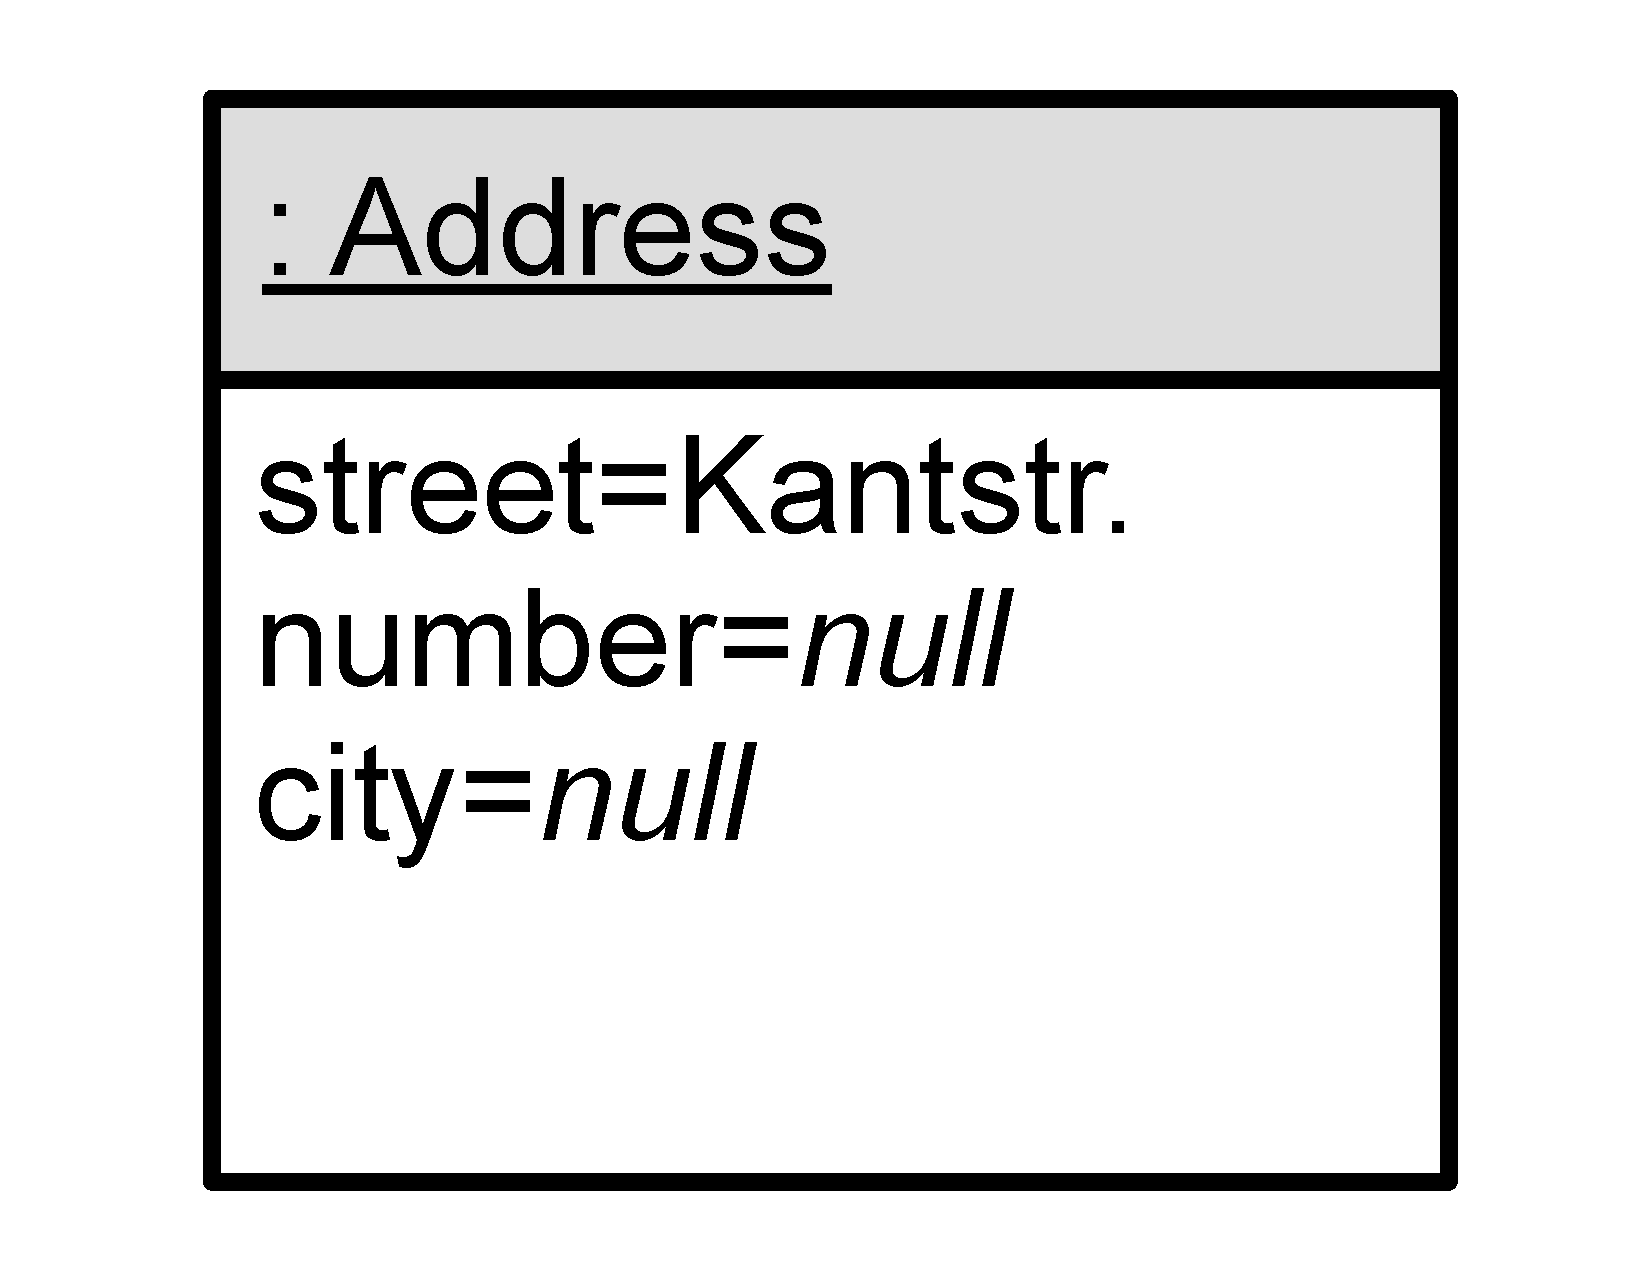
\includegraphics[width=0.22\textwidth]{figures/4_approach/1_singleObject.pdf}
    \caption{An \emph{address} object with three properties.}
    \label{fig:SingleObject}
\end{figure}

If the \lstinline{address} object gets values assigned to its \lstinline{city} and \lstinline{number} fields, the object's state is changed.
As the address object's state is part of the system state, changing the address object changes the system state.
If we call the initial state version \emph{v1} and the state after making changes to the object version \emph{v2}, the state of the address object is different in the two versions of the system, as shown in Figure~\ref{fig:ObjectChanged}.

\begin{figure}[h]
    \centering
    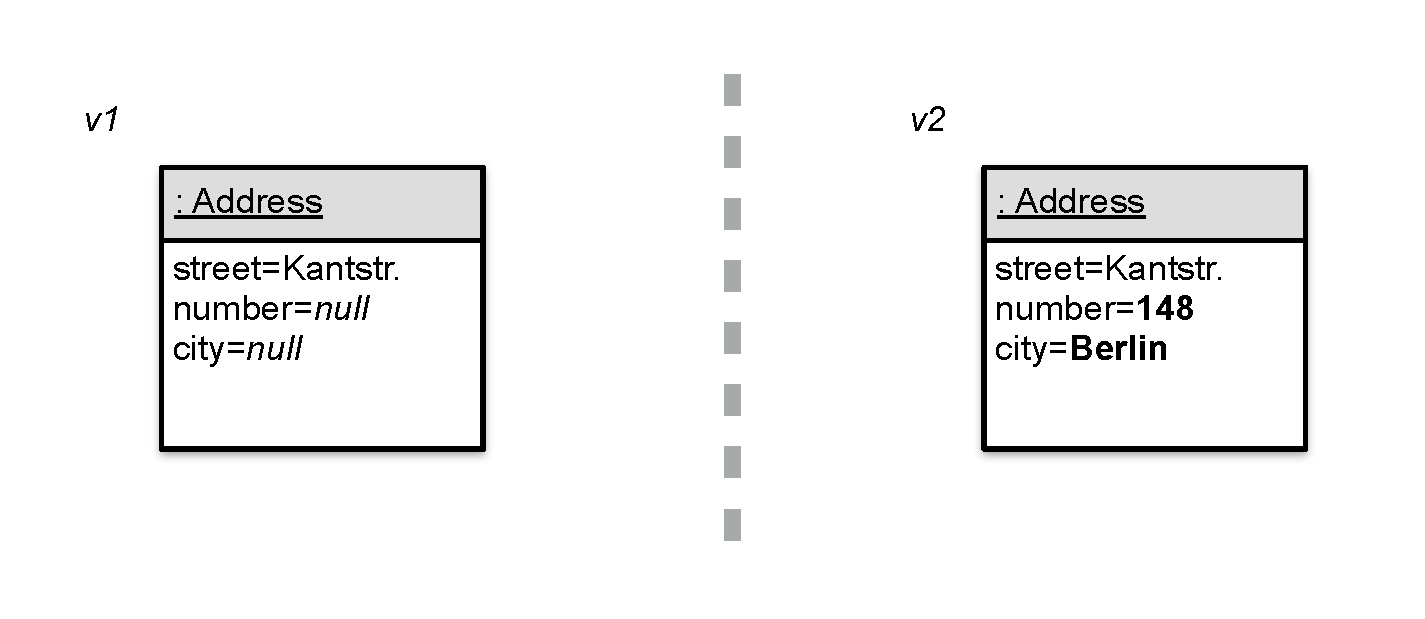
\includegraphics[width=0.7\textwidth]{figures/4_approach/2_objectChange.pdf}
    \caption{Two versions of an \emph{address} object in two versions of the system.}
    \label{fig:ObjectChanged}
\end{figure}

To be able to recover previous versions after making changes, the previous states of objects need to be accessible.
For this reason, versions of objects are preserved and changes are made to new versions of the objects.
A version of an object is, in the simplest case, a copy of an object.
When the \lstinline{address} object is changed in version \emph{v2} of the system, the system does not change the orginal \lstinline{address} object but the copy.

\begin{figure}[h!]
    \centering
    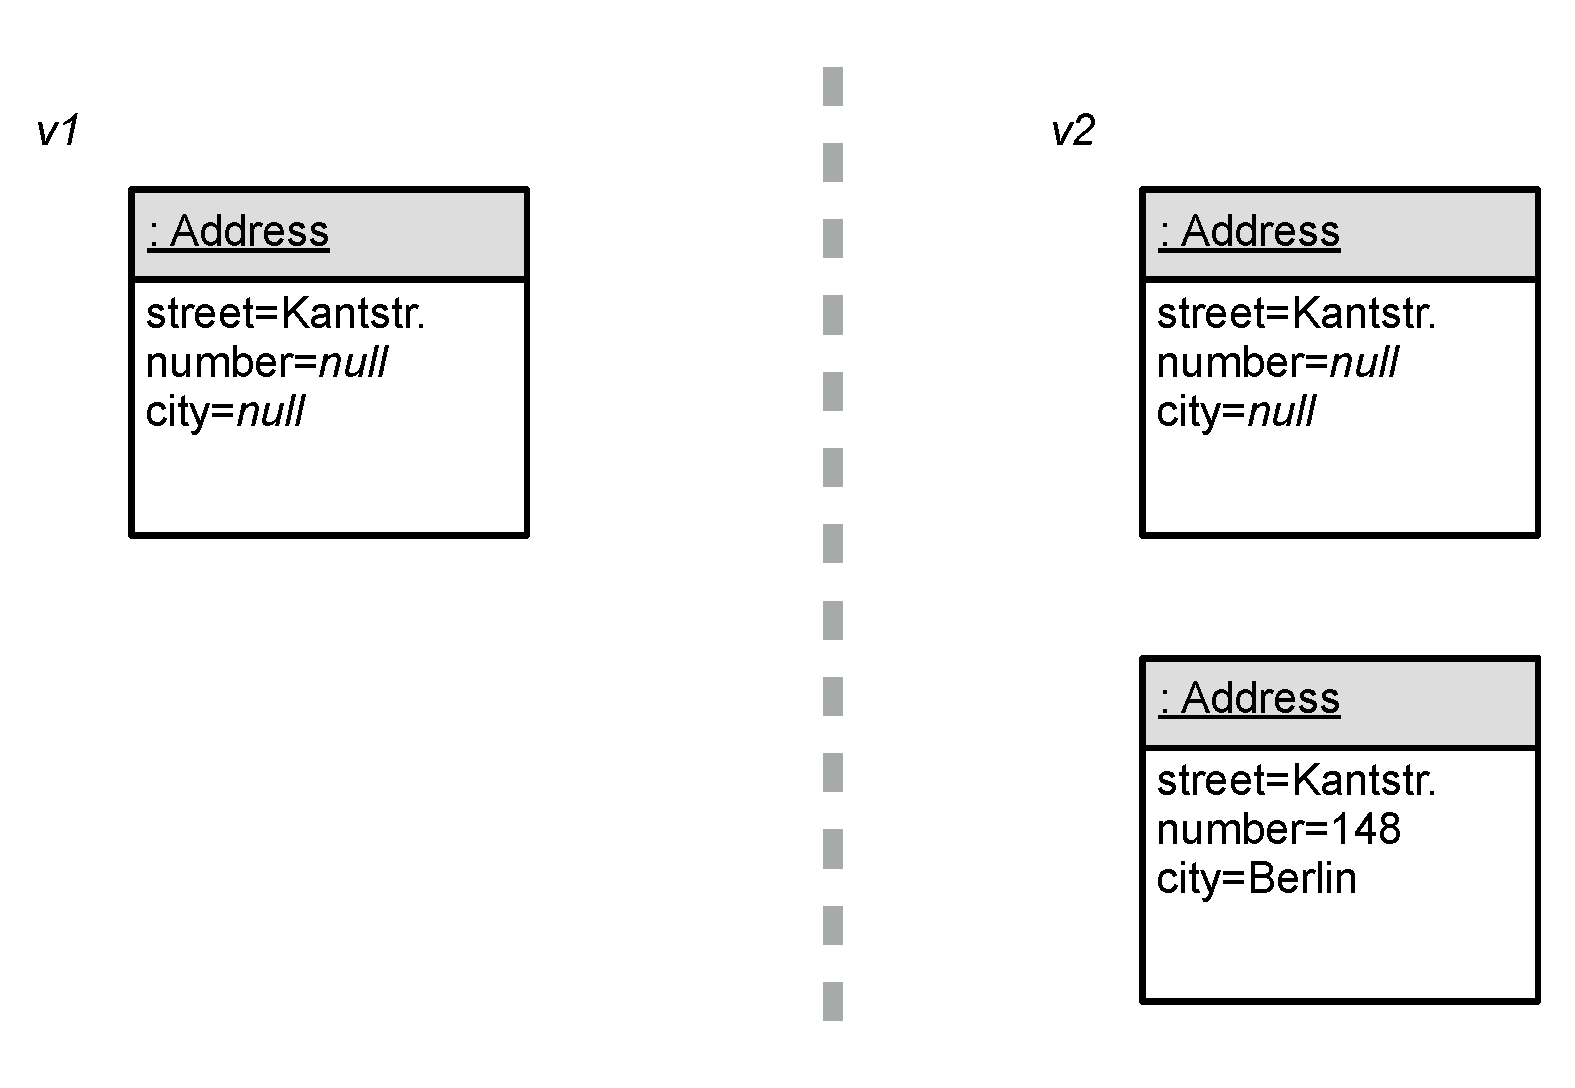
\includegraphics[width=0.7\textwidth]{figures/4_approach/3_previousVersionPreserved.pdf}
    \caption{Preserving the previous version of the \emph{address} object.}
    \label{fig:VersionPreserved}
\end{figure}

As shown in Figure~\ref{fig:VersionPreserved}, there are now two versions of the \lstinline{address} objects in version \emph{v2} of the system.
One of the objects holds the original state, while the other holds the state the object should have in version \emph{v2} of the system.
The two objects hold no information that indicates to which version of the system they belong.
They also store no information that one object is a copy of the other one.
At the same time, references to objects remain unchanged.
For example, there could have been a \lstinline{person} object referring to the \lstinline{address} object.
This reference would still be referring to the original \lstinline{address} object, even in version \emph{v2} of the system, as shown in Figure~\ref{fig:ReferenceFixedToPreviousVersion}.

\begin{figure}[h!]
    \centering
    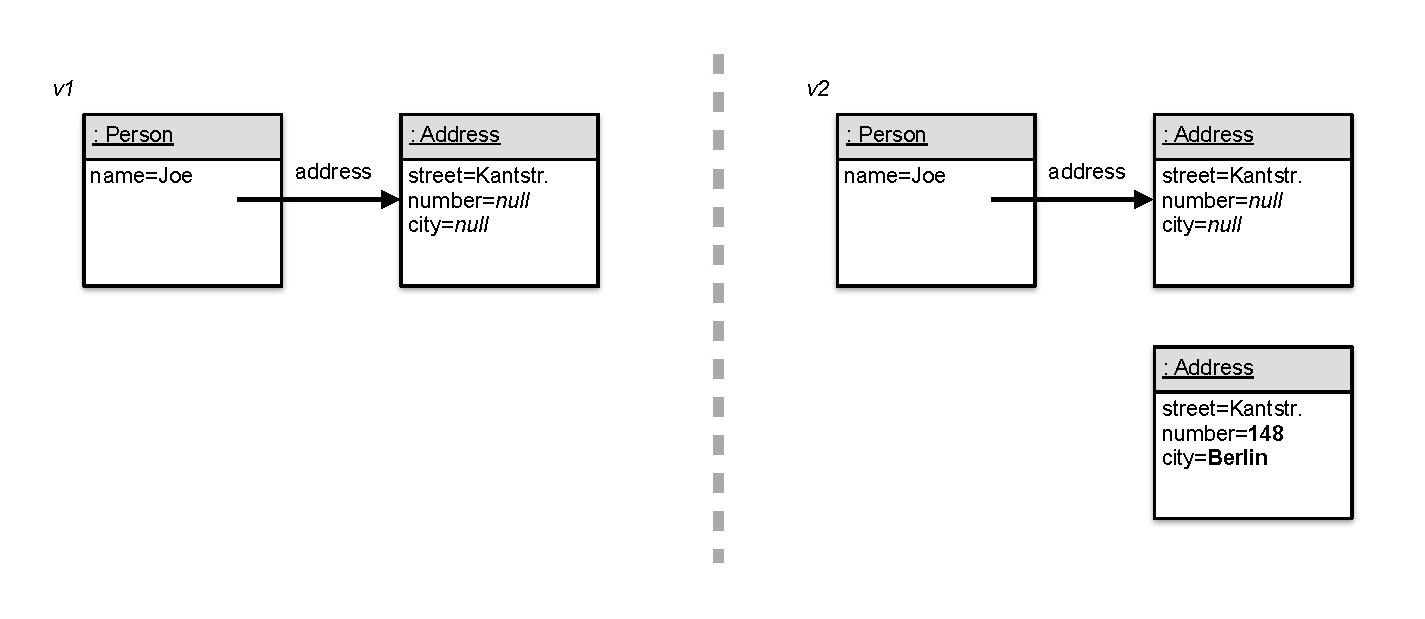
\includegraphics[width=\textwidth]{figures/4_approach/4_referenceToPreviousVersion.pdf}
    \caption{A reference refers to the previous version of the \emph{address} object.}
    \label{fig:ReferenceFixedToPreviousVersion}
\end{figure}

Even after adding values to the fields of the \lstinline{address} object, the following statement would still return \lstinline{true} when \lstinline{aPerson} refers to the \lstinline{person} object:

\iffalse
\begin{verbatim}\fi    
\begin{code}[lst:wrongState]{}{}
aPerson.address.city === null
\end{code}
\iffalse
\end{verbatim}\fi


\subsubsection{Version-aware References}

Our approach uses \emph{version-aware references}.
Version-aware references know the available versions of an object and always resolve to one of those.
Moreover, version-aware references know which version of an object belongs to which version of the system.
Using context information, the version-aware references resolve dynamically to the correct versions.
That is, none of the versions is hard-wired to be the active version.

Otherwise, the version-aware references behave like ordinary references.
They can be assigned to variables, object fields, and are passed around.

When the \lstinline{person} object uses a version-aware reference to refer to its \lstinline{address} property, it can resolve to the versions of its \lstinline{address} object.
The version-aware reference knows both versions of the address object.
In version \emph{v2} of the system, it resolves to the second version of the object, as shown in Figure~\ref{fig:VersionAwareReferenceFollowingVersion2}.

\begin{figure}[h]
    \centering
    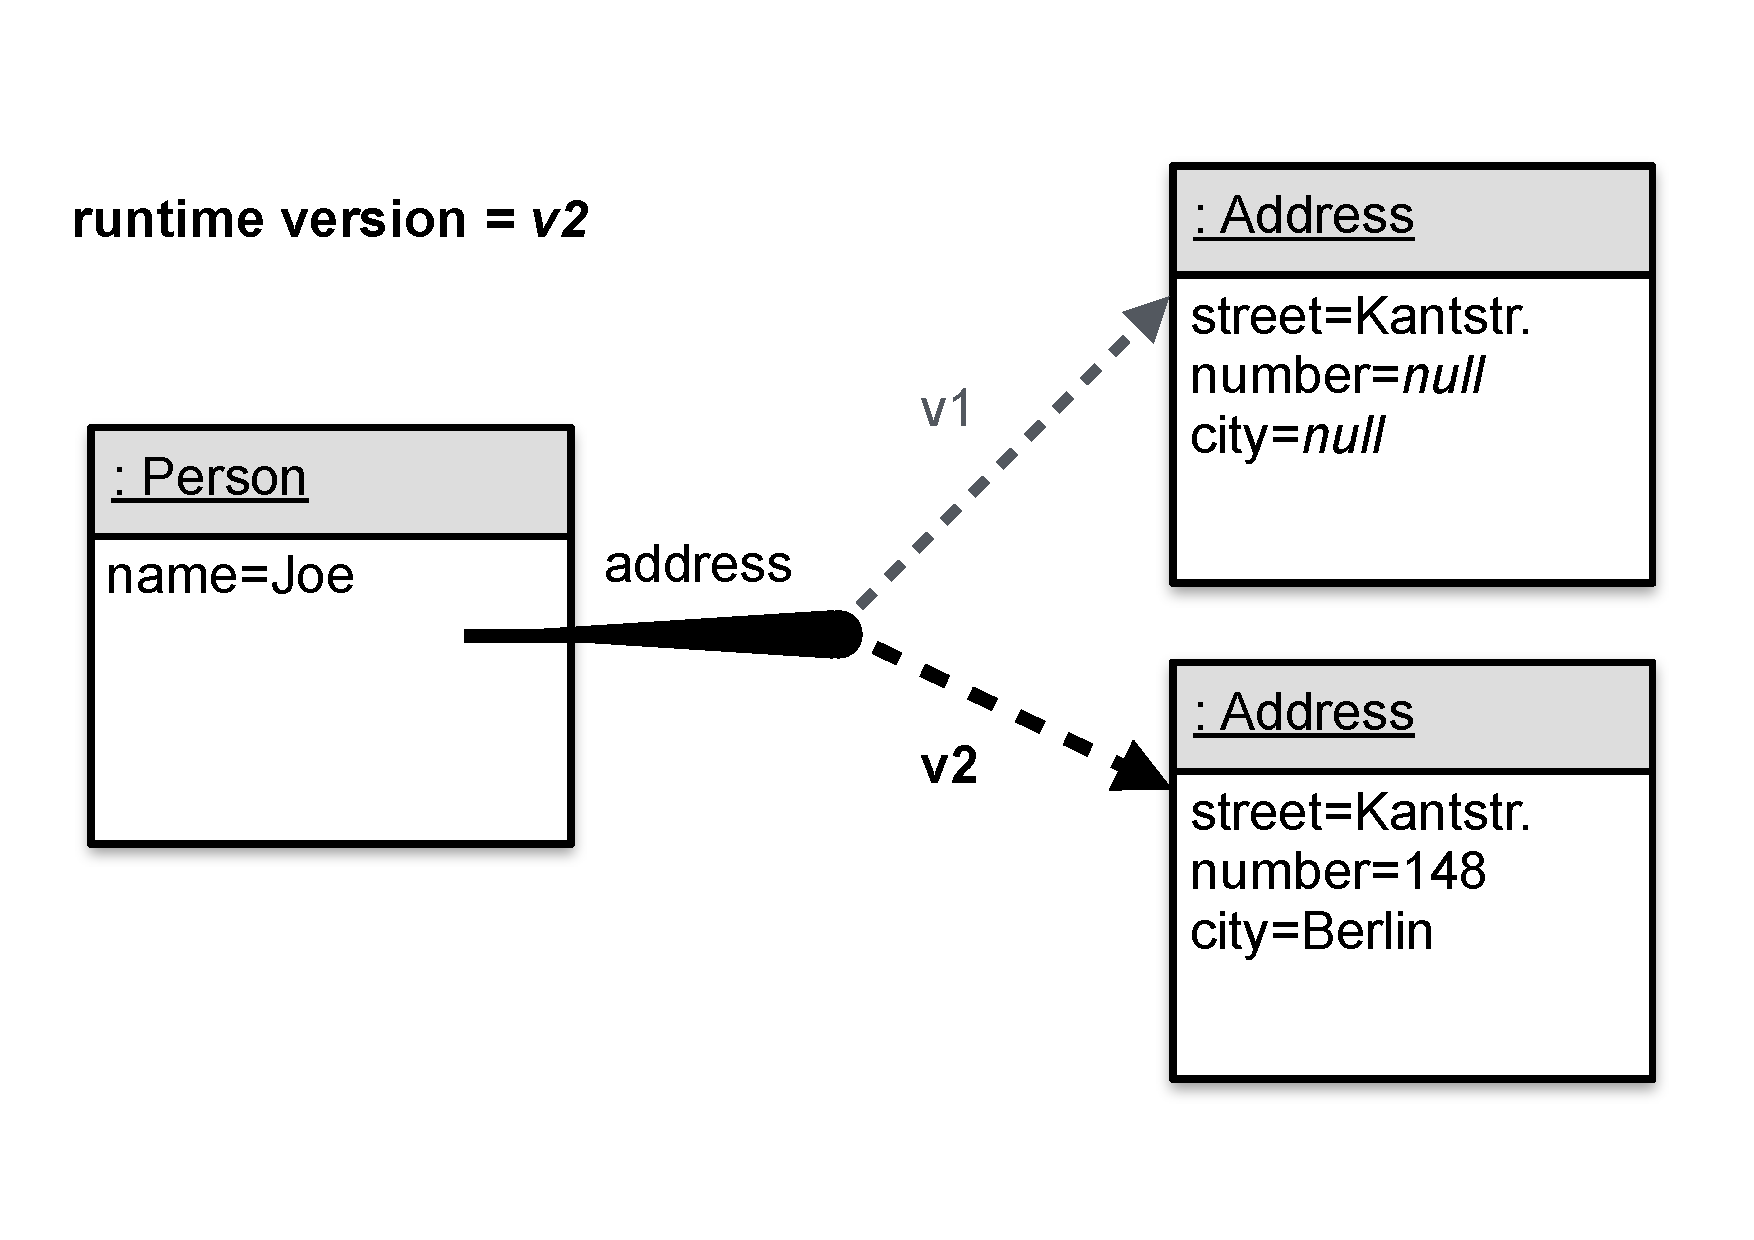
\includegraphics[width=0.8\textwidth]{figures/4_approach/5_versionAwareReferenceFollowingVersion2.pdf}
    \caption{A version-aware reference relates a \emph{person} object to two versions of its \emph{address} property.}
    \label{fig:VersionAwareReferenceFollowingVersion2}
\end{figure}

In the same way, multiple version-aware references can be resolved as one path through a graph of versions.
The version-aware references all choose versions of objects that belong to the same system state and, thereby, form the object graph of that state.

Figure~\ref{fig:ObjectGraphWithReferencesResolvedAlongVersion2} shows an object graph that incorporates the previous example.
The previously presented \lstinline{person} object is a \lstinline{company} object's \lstinline{CEO} property.
While the example shows that version \emph{v2} is active, it also indicates a version \emph{v1} and a version \emph{v2} of the system.
In version \emph{v1}, the company's CEO has incomplete address information.
In version \emph{v3}, the company has a different CEO.

\begin{figure}[h]
    \centering
    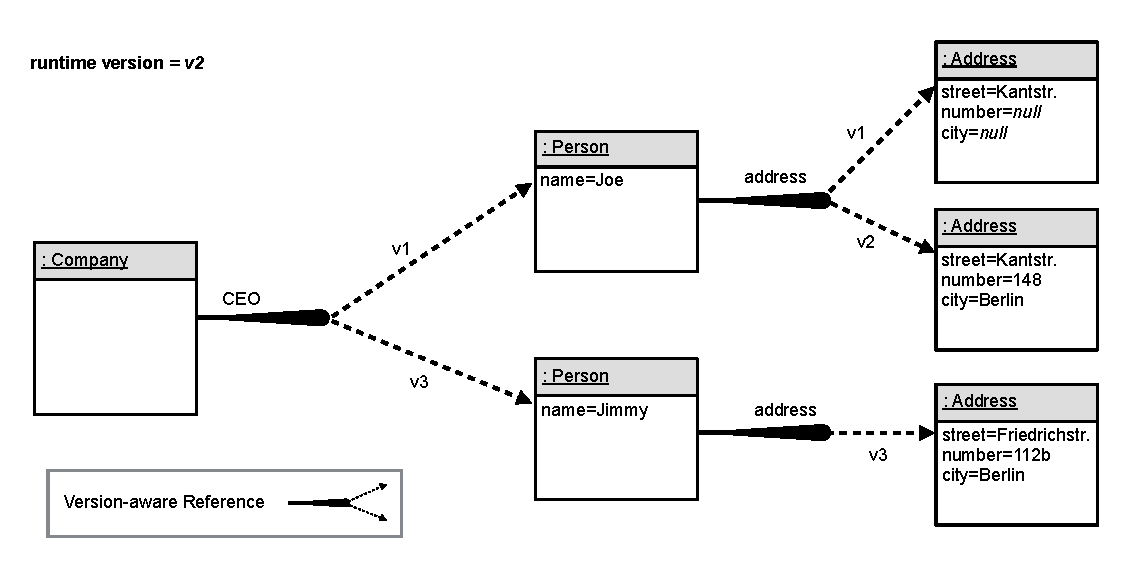
\includegraphics[width=\textwidth]{figures/4_approach/6_objectGraphWithVersonAwareReferences.pdf}
    \caption{Three versions of a \emph{company} object, in which objects are connected through version-aware references.}
    \label{fig:ObjectGraphWithReferencesResolvedAlongVersion2}
\end{figure}


\subsubsection{Versions of the System}

To establish different versions of the system, the version-aware references have to resolve to different versions of objects.
The version-aware references choose versions dynamically following a \emph{version identifier}.
Only this version identifier has to be changed to have version-aware references resolve to other versions of objects.
For example, to undo the changes made with version \emph{v2} of the system, the version identifier would need to be set to \emph{v1} again.

Given the example situation from Figure~\ref{fig:ObjectGraphWithReferencesResolvedAlongVersion2} and given \lstinline{aCompany} refers to the \lstinline{company} object, the following statement would refer to three different values depending on the version identifier:

\iffalse
\begin{verbatim}\fi
\begin{code}[lst:example]{}{}
aCompany.CEO.address.number
\end{code}
\iffalse
\end{verbatim}\fi

Evaluating the statement in version \emph{v1} would return the value \lstinline{null}, in version \emph{v2} the value \lstinline{148}, and in version \emph{v3} the value \lstinline{112b}.

The information that one version is the predecessor of another version can be used to resolve to the an earlier version of an object when current version is available.
This allows to only create new versions of objects when necessary.

The version identifier needs to be accessible to the version-aware references.
It could be available globally, to have a single active version of the system, but could also be scoped more locally such as thread-local or in the dynamic scope of a code block.
It should, however, not be changed while multiple version-aware references of an object graph are resolved transitively.
That is, the version-aware references involved in evaluating the previous example statement should be resolved together for the same version identifier.

To be able to actually re-establish a particular version of the system with our approach, two requirements need to be fullfilled:
First, all mutable objects of the programming runtime need to be accessed via version-aware references.
Second, the particular version of the system needs to be available.
That is, not every state is recoverable, but specific states have to be preserved.
Programmers could preserve versions explicitly or the programming system could do this implicitly.
When the programming system automatically preserves versions, each programmer action could implicitly yield a new version of the system.
This way, programmers could undo and redo the changes of their actions regardless of whether they preserved a version in anticipation of recovery needs or not.

\subsubsection{Discussion}

The version-aware references allow to preserve and re-establish versions of the system without completely halting the program execution.
That is, the presented approach is incremental, not a stop-the-world approach.\\
First, the version-aware references resolve dynamically to particular versions based on context information.
Only this context information has to be changed to have all references resolve to another version.
The version-aware references do not have to be re-configured individually.\\
Second, versions of the system are preserved incrementally.
Instead of saving the state of all objects the moment a version is preserved, new versions of objects are created only when objects change.
Before such writes, previous object versions continue to reflect the current state and can be read until written to.


\section{Using Proxies as Version-aware References} \label{sec:APPROACH:2}

We used proxies to implement version-aware references in JavaScript.
Instead of actually requiring \emph{alternative references}, proxies are referred to by \emph{ordinary references} and transparently delegate to versions. 
This way, proxies allow a language-level implementation of version-aware references that works with existing JavaScript engines.

\subsubsection{Proxies as Version-aware References}

Figure~\ref{fig:ProxyBasedVersionAwareReference} exemplifies how a proxy implements a version-aware reference in our solution.
The proxy connects a \lstinline{person} object to the two versions of its \lstinline{address} property.
The \lstinline{person} holds an ordinary reference to the proxy in its \lstinline{address} slot.
The proxy in turn knows which versions are available for the \lstinline{address} object.

\begin{figure}[h]
    \centering
    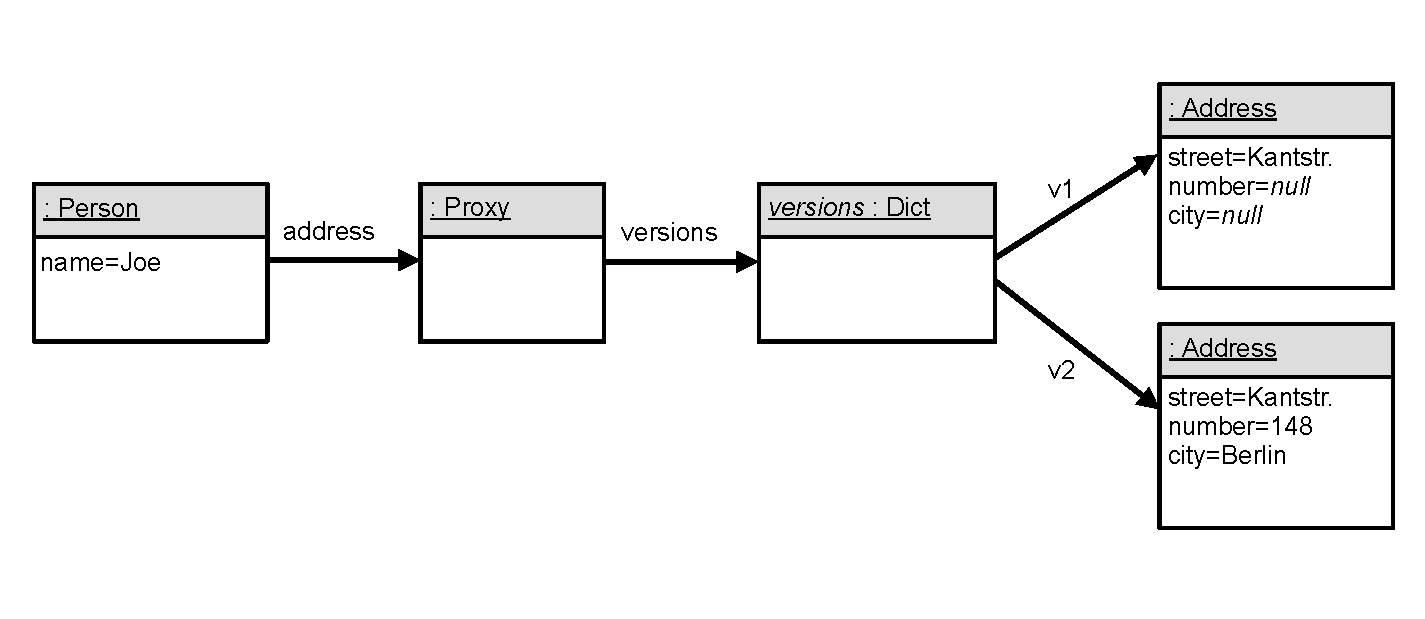
\includegraphics[width=\textwidth]{figures/4_approach/7_proxyBasedVersionAwareReference.pdf}
    \caption{Using a proxy as version-aware reference to connect a \emph{person} object with two versions of an \emph{address} object.}
    \label{fig:ProxyBasedVersionAwareReference}
\end{figure}

When the \lstinline{address} property of the \lstinline{person} object is accessed, the proxy forwards the access transparently to a version.
For example, in version \emph{v2} of the system as indicated by Figure~\ref{fig:ProxyBasedVersionAwareReference}, even if the \lstinline{address} property is a proxy, reading the proxy's \lstinline{city} property returns the string \lstinline{'Berlin'} .
Given \lstinline{aPerson} refers to the \lstinline{person} object, evaluating the following statement returns \lstinline{true} in version \emph{v2}:

\iffalse
\begin{verbatim}\fi
\begin{code}[lst:example]{}{}
aPerson.address.city === 'Berlin'
\end{code}
\iffalse
\end{verbatim}\fi

The statement does not include any version information.
In particular, it does not read a specific version from a table of available versions.
Instead, the proxies intercept all object interactions and forward to specific versions transparently.

The proxies fulfill three responsibilities:
\begin{enumerate}
    \item They know which versions are available for a particular object.
    \item They choose a particular version among all available dynamically using context information.
    \item They forward all interactions transparently to a chosen version.
\end{enumerate}

The proxies required by this design are \emph{virtual objects}~\cite{VanCutsem2010PDP}.
They do not stand in for specific objects, but can forward intercepted interactions to any object.


\subsubsection{Using Proxies Consistently}

The proxies need to be used consistently for all mutable state.
Ordinary references that usually refer to an object need to refer to the proxy that stands in for the object.

To use proxies consistently, we create and return proxies for all new objects.
All expressions that create new objects return proxies for those objects instead.
This is achieved by transforming code before it is executed.
The source transformations wrap object literals and constructor functions into proxies.
The proxies also always return proxies as return values.
Thus, when proxied constructors are used, the constructors return proxies for the new objects.

The reference to the initial version of an object is only available to the proxy.
The reference to the proxy gets passed around instead.
For this reason, all references that would usually point to the same object point to the same proxy.
This way, proxies provide object identity.
Checks that would usually compare an object to another objects now compare a proxy to another proxy.

As only the proxies hold references to the versions of objects, the versions get garbage collected with the proxies when the proxies are no longer reachable.
For example, in the code of Listing~\ref{lst:deletedAddress}, there would temporarily exist a version-aware reference---a proxy---connecting the \lstinline{person} object to an \lstinline{address} object, but the reference gets deleted before a version of the system is preserved.
The \lstinline{address} object is not required to re-establish either version \emph{1} or version \emph{2} of the system and nothing does prevent the garbage collector from reclaiming the proxy for the \lstinline{address} object with the \lstinline{address} object.

\iffalse
\begin{verbatim}\fi
\begin{code}[lst:deletedAddress]{A newly created object is not preserved with any version.}{float,numbers=left}
    var person = {name: "Joe"};
    
    \\ [preserve first version]
    
    person.address = {street: "Kantstr.",
                      number: "148",
                      city: "Berlin"};
    
    delete person.address;
    
    \\ [preserve second version]
\end{code}
\iffalse
\end{verbatim}\fi


\subsubsection{Versions of the System}

Proxies delegate to and create versions of an object using a \emph{version of the system}.

A version of the system is an object that has a \emph{version identifier}, a \emph{predecessor} version, and a \emph{successor} version.
Figure~\ref{fig:SystemVersions} shows three system versions.
In the example, version \emph{v2} is the current version of the system.

\begin{figure}[h]
    \centering
    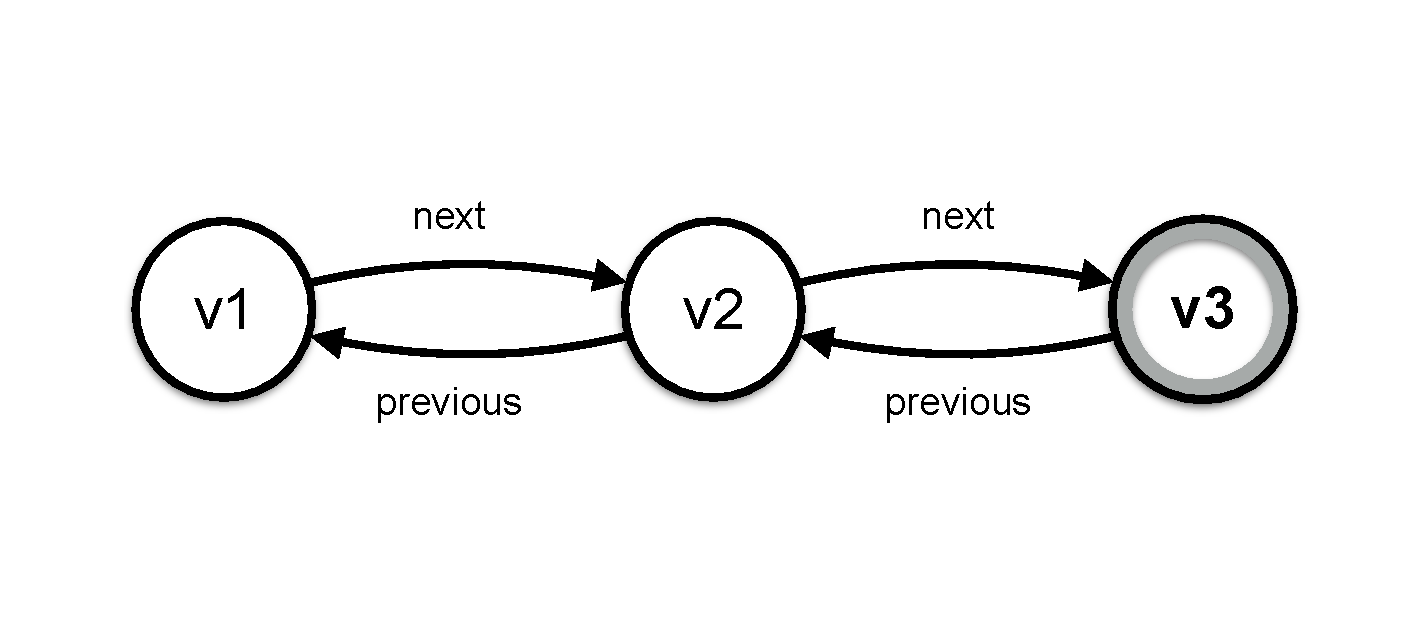
\includegraphics[width=0.65\textwidth]{figures/4_approach/8_systemVersions.pdf}
    \caption{Four objects representing four linear versions of the system.}
    \label{fig:SystemVersions}
\end{figure}

The current version of the system is accessible to the proxies.
Proxies use it to decide to which version of an object they currently should forward to.
Figure~\ref{fig:ProxyUseSystemVersion} shows a proxy with \emph{versions of an object} in the context of \emph{versions of the system}.
In this example, there are two object versions that correspond to the two system versions.
The current version of the system is \emph{v2} and, therefore, the version the proxy currently forwards to is version \emph{v2} of the object.

\begin{figure}[h]
    \centering
    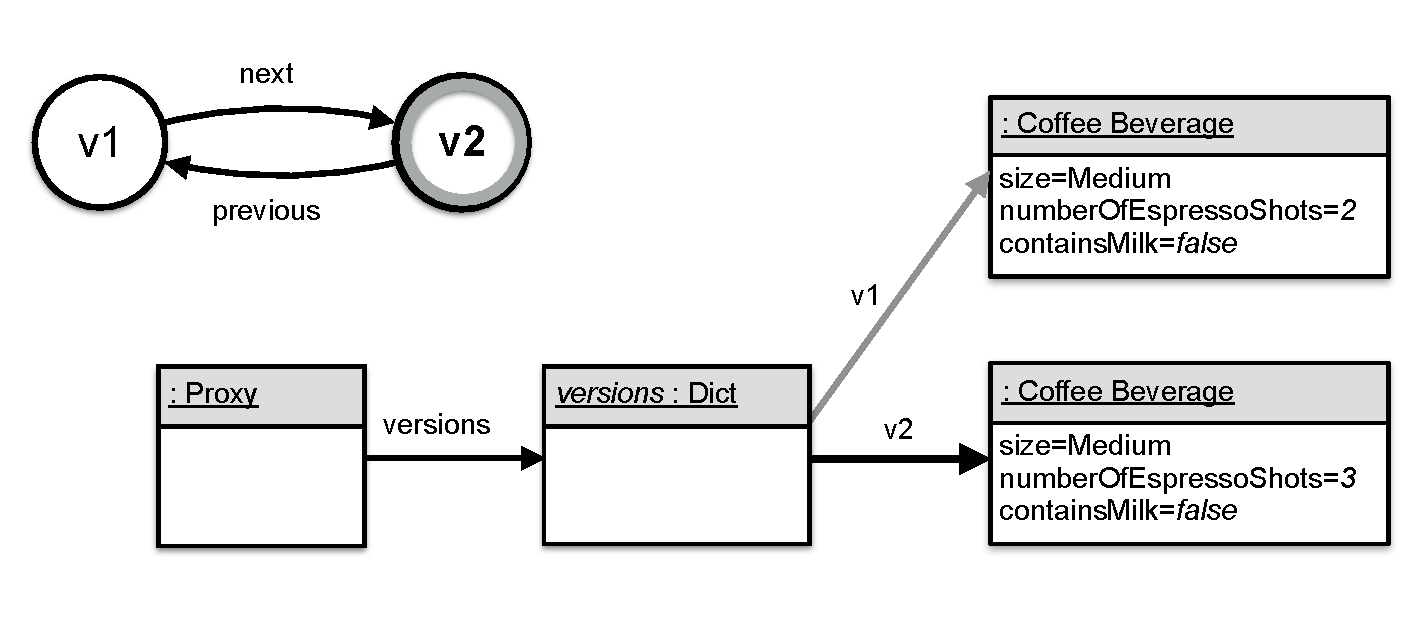
\includegraphics[width=\textwidth]{figures/4_approach/9_proxyUsesSystemVersion.pdf}
    \caption{A proxy with two versions of an object in context of the versions of the system.}
    \label{fig:ProxyUseSystemVersion}
\end{figure}

As long as the system version stays the same, the proxies forward to the same version of the object.
Therefore, an object version is changed only as long it the current system versions matches.

\emph{To re-establish the previous version}, the current system version has to be set to its predecessor.
In that case, proxies forward interactions to previous versions of the objects.

\emph{To preserve the current version}, the current system version has to be set to another version.
The proxies forward interactions to objects of the other version or, when no such version of the object exist, create new versions.

\begin{figure}[h]
    \centering
    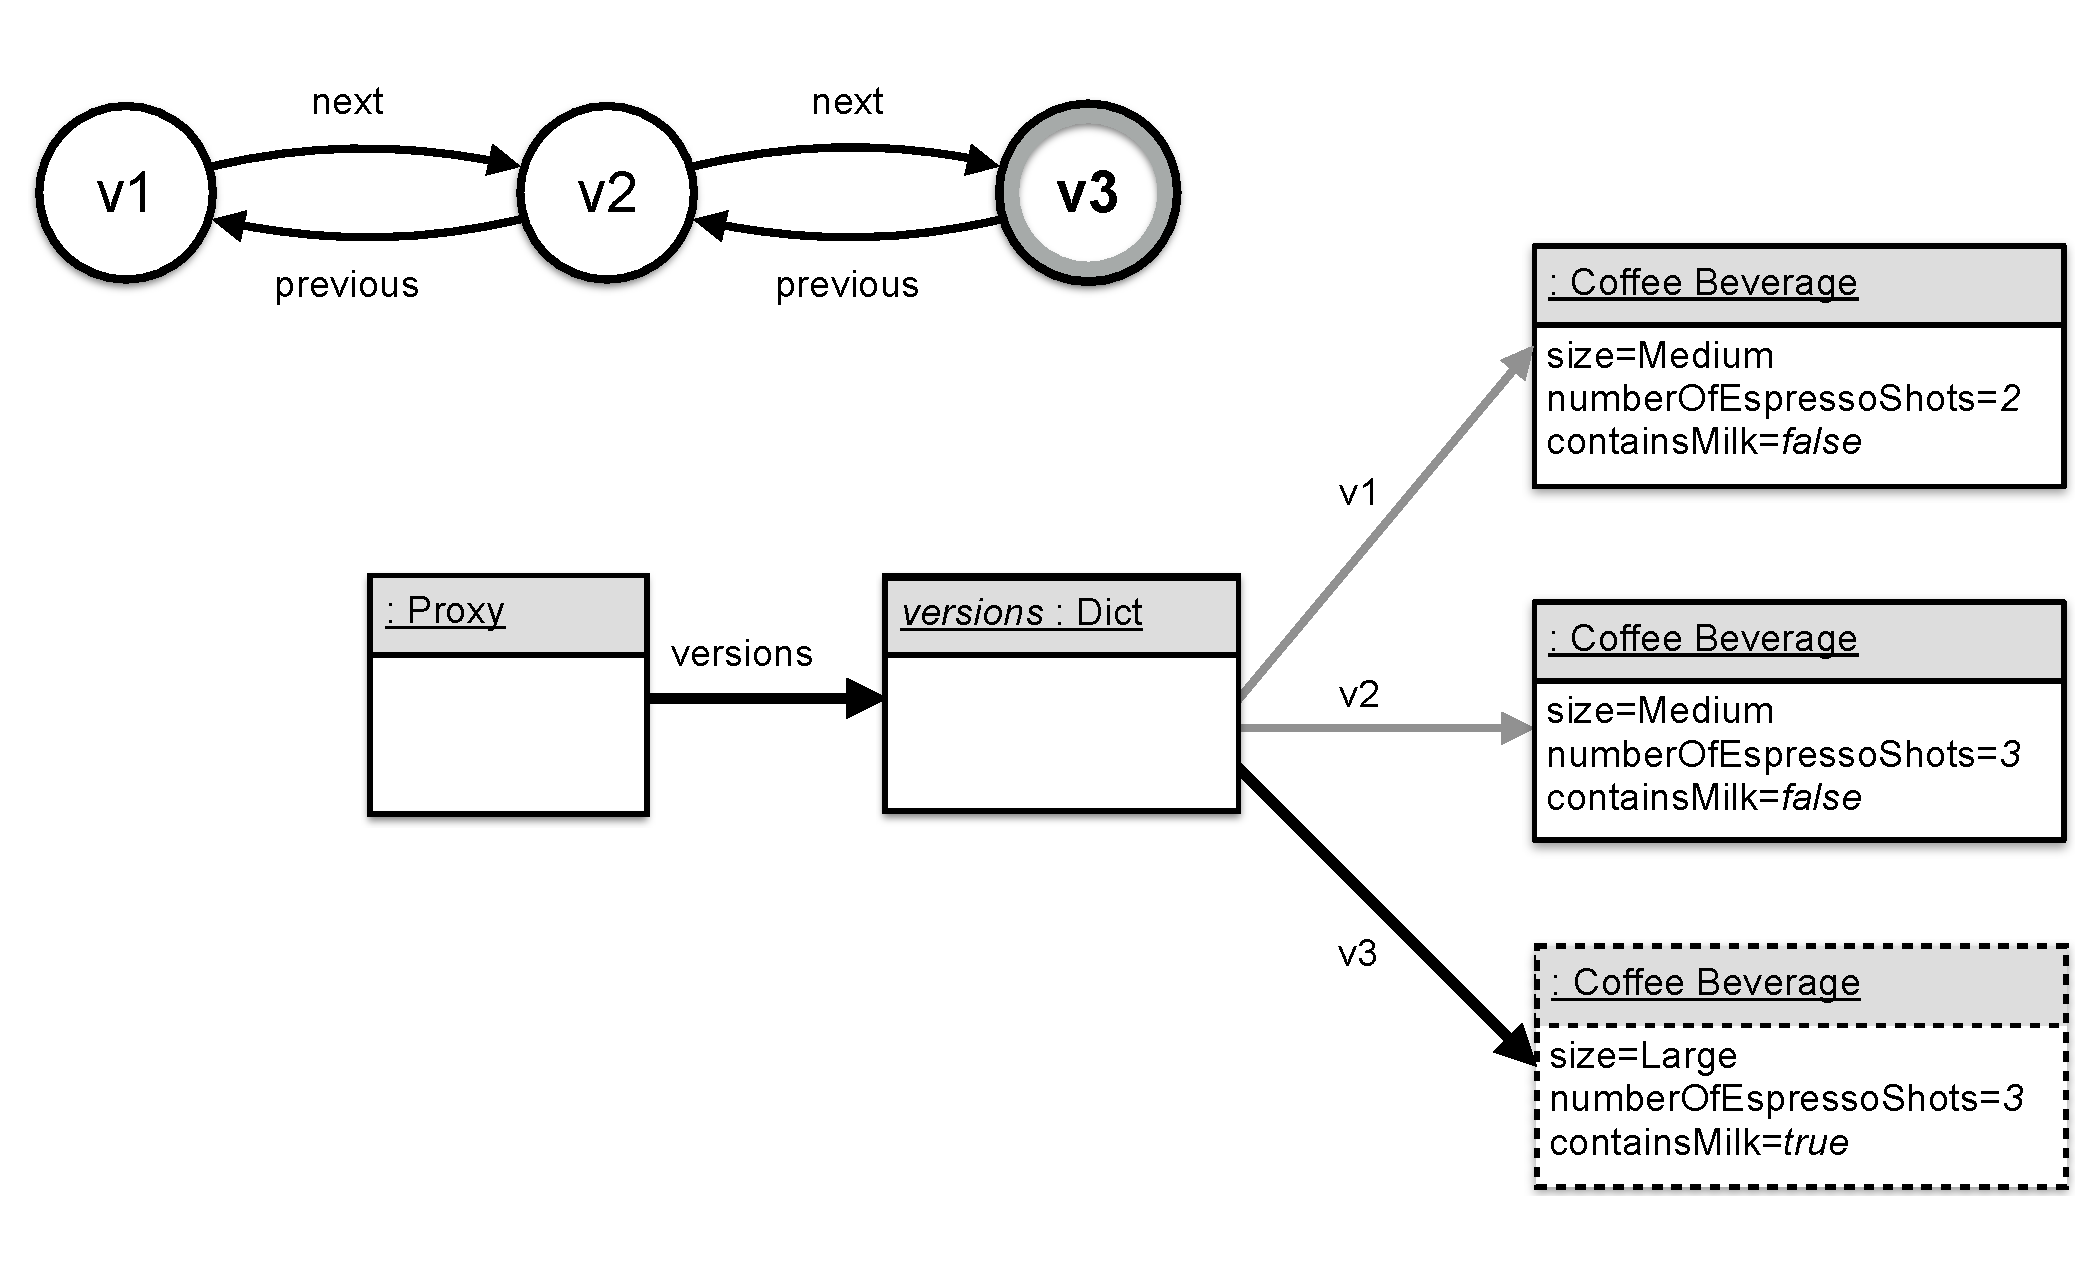
\includegraphics[width=0.86\textwidth]{figures/4_approach/10_newVersionOfAnObject.pdf}
    \caption{A new version of an object needs is created for a new version of the system.}
    \label{fig:NewVersion}
\end{figure}

A situation in which a new version of an object is created is shown in Figure~\ref{fig:NewVersion}.
In a new version \emph{v3} of the system, the proxy intercepts a manipulation but has no object version it can forward to.
It, therefore, copies the most recent version of the object and forwards to the copy.

New versions are only necessary when a proxy is about to delegate manipulations.
As long as the state of an object is only read, the proxy reports values from a previous version as the old version of the object still reflects the current state.
To create a new version, a proxy copies the most recent previous version of the object.


\subsubsection{Limitations}

The current design allows to preserve and re-establish versions of the system.
Without further components, however, these versions only exist in memory and are not stored to disk.

Our current design does not support multiple predecessors or successors.

Another limitation of the current design is that the state of previous versions can be changed.
New versions of objects are not affected by changes to previous versions, but changes to object versions that have not been copied shine through in subsequent versions of the system.

In the future, the versioning might allow for branches and merging.
Changes to previous states could then be handled in branches that programmers may or may not merge into future versions.
